\documentclass{beamer}
\usetheme{Warsaw}
\title{Numerical Python for Scalable Architectures}
\author{Mads Ruben Burgdorff Kristensen \and Brian Vinter}
\institute{eScience Centre\\ University of Copenhagen\\ Denmark\\ madsbk@diku.dk/vinter@diku.dk}
\date{May 12, 2010}


\begin{document}
\begin{frame}
\titlepage
\end{frame}

%%%%%%%%%%%%%%%%%%%%%%%%%%% FRAME %%%%%%%%%%%%%%%%%%%%%%%%%%%

\begin{frame}{Outline}
\begin{itemize}
\item Motivation
\item Python
\item Numerical Python (NumPy)
\item DistNumPy
\item Benchmarks
\end{itemize}
\end{frame}

%%%%%%%%%%%%%%%%%%%%%%%%%%% FRAME %%%%%%%%%%%%%%%%%%%%%%%%%%%

\begin{frame}{Motivation -- Workflow}
\begin{center}
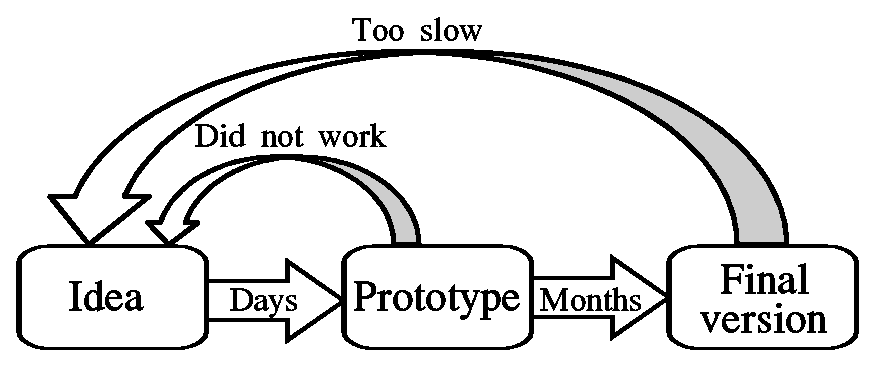
\includegraphics[width=150px]{../gfx/workflow1}
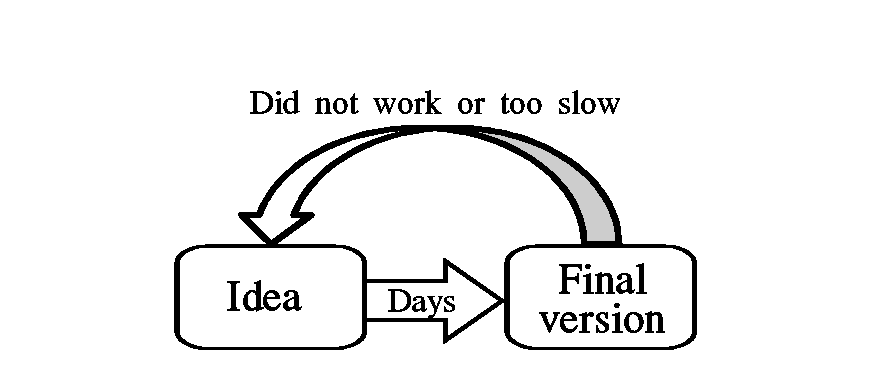
\includegraphics[width=150px]{../gfx/workflow2}
\end{center}
\begin{itemize}
\item High Productivity
  \begin{itemize}
    \item High-level language
    \item No compilation
    \item Interactive
  \end{itemize}
\item High Performance
  \begin{itemize}
    \item Low-level language such as C, Fortran, etc.
    \item Compiling to machine code
    \item Highly Optimized Compilers
    \item Parallel Programming
  \end{itemize}
\end{itemize}
\end{frame}

%%%%%%%%%%%%%%%%%%%%%%%%%%% FRAME %%%%%%%%%%%%%%%%%%%%%%%%%%%

\begin{frame}{Python}
\begin{center}
\begin{Large}
Python
\end{Large}
\end{center}
\begin{itemize}
\item General-purpose high-level programming language
\item The design philosophy emphasizes code readability.
\item Sacrificing performance over productivity
%\item Commenly used for: ad-hoc programming, prototyping 
\item Gluing libraries together
\end{itemize}
\end{frame}

%%%%%%%%%%%%%%%%%%%%%%%%%%% FRAME %%%%%%%%%%%%%%%%%%%%%%%%%%%

\begin{frame}[fragile]{Numerical Python}
\begin{center}
\begin{Large}
Numerical Python (NumPy)
\end{Large}
\end{center}
\begin{itemize}
  \item Framework for numerical computation similar to Matlab
  \item Introduces efficient arrays and a lot of useful array operations
\begin{itemize}
  \item Linear algebra functions
  \item Fourier transforms
  \item Random number arrays  
\end{itemize}
\end{itemize}
\begin{center}
\includegraphics[width=80px]{SoftwareLayout}
\end{center}
\end{frame}

%%%%%%%%%%%%%%%%%%%%%%%%%%% FRAME %%%%%%%%%%%%%%%%%%%%%%%%%%%

\begin{frame}[fragile]{Universal Functions}
\begin{center}
Vectorized operations called Universal Functions
\end{center}
\begin{scriptsize}
\begin{verbatim}

         #C                                #Python
         for(i = 0; i < rows; i++)         c = []
             c[i] = a[i] + b[i];             for i in range(len(a)):
                                               c.append(a[i] + b[i])
         #NumPy
         c = a + b
\end{verbatim}
\end{scriptsize}
\end{frame}

%%%%%%%%%%%%%%%%%%%%%%%%%%% FRAME %%%%%%%%%%%%%%%%%%%%%%%%%%%

\begin{frame}[fragile]{Broadcast}
\begin{center}
Matching arrays that have different dimensions
\end{center}
\begin{scriptsize}
\begin{verbatim}
                        #No broadcast
                        for i in range(len(A)):
                            c[i] = a[i] + b
                  
                        #Broadcast
                        c = a + b
\end{verbatim}
\end{scriptsize}
\begin{center}
\includegraphics[width=100px]{../gfx/ufunc_broadcast}
\end{center}
\end{frame}

%%%%%%%%%%%%%%%%%%%%%%%%%%% FRAME %%%%%%%%%%%%%%%%%%%%%%%%%%%

\begin{frame}{DistNumPy}
\begin{center}
\begin{Huge}
DistNumPy
\end{Huge}

\vspace{7px}
A distributed version of NumPy

\vspace{25px}
\begin{scriptsize}
Ideal workflow -- High Productivity and High Performance
\end{scriptsize}
\end{center}
\end{frame}

%%%%%%%%%%%%%%%%%%%%%%%%%%% FRAME %%%%%%%%%%%%%%%%%%%%%%%%%%%

\begin{frame}[fragile]{Transparent parallelism}
\begin{itemize}
  \item DistNumPy introduces a distributed parallel array-backend
  \item Still sequential programming
  \item Parallel execution of universal functions
\end{itemize}
\vspace{15px}
\begin{center}
\begin{small}
Monte Carlo $\pi$ simulation
\end{small}
\begin{scriptsize}
\begin{verbatim}
          from numpy import *
          S = 1000 #Number of samples
          (x, y) = (empty([S], dist=True), empty([S], dist=True))
          (x, y) = (random(x), random(y))
          (x, y) = (square(x), square(y))
          z = (x + y) < 1
          print add.reduce(z) * 4.0 / S #The result
\end{verbatim}
\end{scriptsize}
\end{center}
\end{frame}

%%%%%%%%%%%%%%%%%%%%%%%%%%% FRAME %%%%%%%%%%%%%%%%%%%%%%%%%%%

%\begin{frame}{Views}
%\begin{center}
%Views\vspace{15px}

%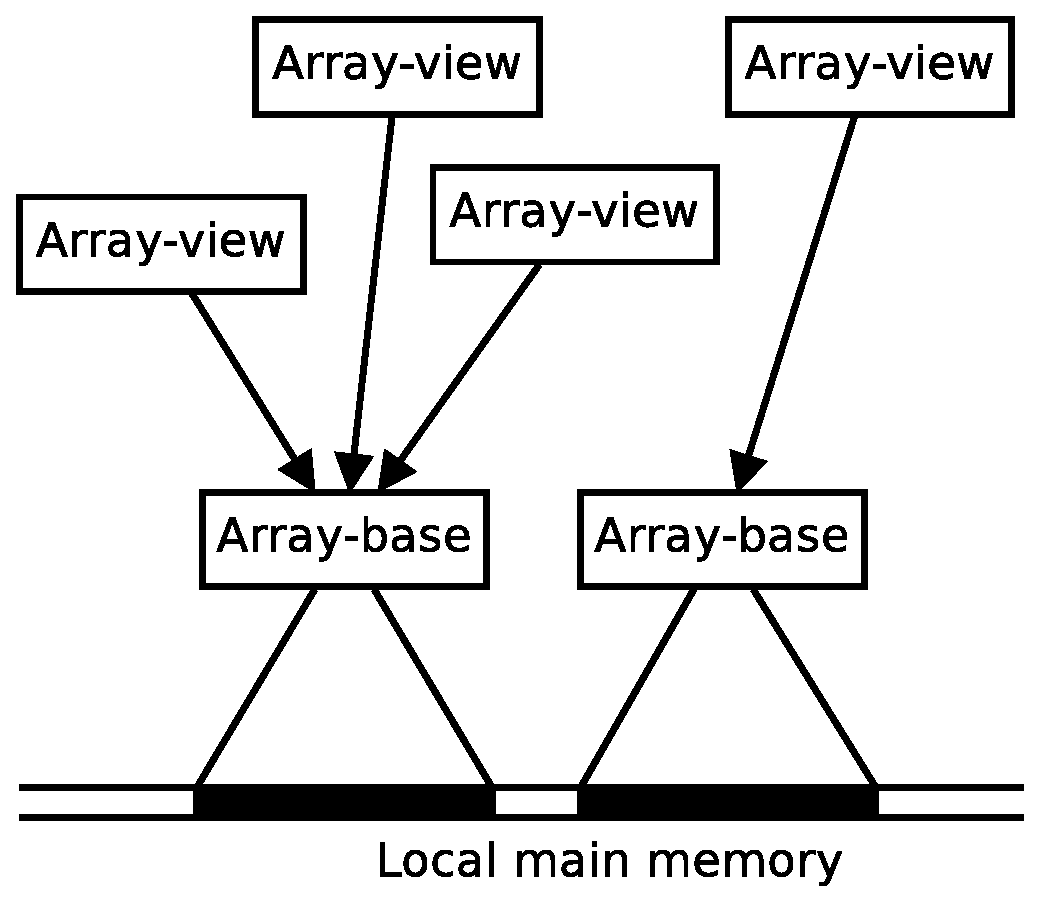
\includegraphics[width=250px]{../gfx/views}
%\end{center}
%\end{frame}

%%%%%%%%%%%%%%%%%%%%%%%%%%% FRAME %%%%%%%%%%%%%%%%%%%%%%%%%%%

\begin{frame}{Data layout}
\begin{center}
N-Dimensional Block Cyclic Distribution\vspace{15px}

\includegraphics[width=250px]{../gfx/datalayout}
\end{center}
\begin{itemize}
  \item Used in High Performance Fortran
  \item Diagonal workflow e.g. Gaussian elimination
\end{itemize}
\end{frame}

%%%%%%%%%%%%%%%%%%%%%%%%%%% FRAME %%%%%%%%%%%%%%%%%%%%%%%%%%%

\begin{frame}{Communication}
\begin{itemize}
  \item DistNumPy make use of MPI version 2.1
  \item One-sided, two-sided and collective communication
  \item Latency hiding by double buffering
\end{itemize}
\end{frame}

%%%%%%%%%%%%%%%%%%%%%%%%%%% FRAME %%%%%%%%%%%%%%%%%%%%%%%%%%%

\begin{frame}{Benchmarks -- Hardware}
\begin{center}
%Hardware\vspace{15px}
\end{center}

\begin{table}
\caption{Hardware specifications}
\centering
\begin{tabular}{|lll|}
\hline
CPU & Core 2 Quad & Nehalem\\
CPU Frequency & 2.26 GHz & 2.66 GHz\\
CPU per node & 1 & 2\\
Cores per CPU & 4 & 4\\
Memory per node & 8 GB @ 6.5 GB/s & 24 GB @ 25.6 GB/s\\
Number of nodes & 8 & 8\\
Network & Gigabit Ethernet & Gigabit Ethernet\\
\hline
\end{tabular}
\label{tab:specs}
\end{table}
\end{frame}

%%%%%%%%%%%%%%%%%%%%%%%%%%% FRAME %%%%%%%%%%%%%%%%%%%%%%%%%%%

\begin{frame}{Scalability}
\begin{center}
%\begin{small}
Monte Carlo $\pi$ simulation
%\end{small}

\vspace{10px}
\includegraphics[width=160px]{../gfx/MonteCarloStrong}
\vspace{3px}

\begin{scriptsize}
Nehalem -- CPU utilization of 88\% on 64 CPU-cores
\end{scriptsize}
\end{center}

\end{frame}

%%%%%%%%%%%%%%%%%%%%%%%%%%% FRAME %%%%%%%%%%%%%%%%%%%%%%%%%%%

\begin{frame}[fragile]{Jacobi solver}
\begin{center}
Jacobi.py
\end{center}
\begin{scriptsize}
\begin{verbatim}
              h = zeros(shape(B), float, dist=True)
              dmax = 1.0
              AD = A.diagonal()
              while(dmax > tol):
                  hnew = h + (B - add.reduce(A * h, 1)) / AD
                  tmp = absolute((h - hnew) / h)
                  dmax = maximum.reduce(tmp)
                  h = hnew
              print h #The result
\end{verbatim}
\end{scriptsize}
\end{frame}

%%%%%%%%%%%%%%%%%%%%%%%%%%% FRAME %%%%%%%%%%%%%%%%%%%%%%%%%%%

\begin{frame}{Scalability -- Jacobi Solver}
\begin{scriptsize}
\begin{columns}
  \begin{column}{0.5\textwidth}
  \begin{center}
    \hspace{21px}Full Cluster
    \includegraphics[width=150px]{../gfx/JacobiStrong}
  \end{center}
  \end{column}
  \begin{column}{0.5\textwidth}
  \begin{center}
    \hspace{23px}Zoomed in
    \includegraphics[width=150px]{../gfx/JacobiStrongSMP}
  \end{center}
  \end{column}
\end{columns}
\begin{center}
Nehalem -- CPU utilization of 85\% on 16 CPU-cores and 50\% on 64 CPU-cores
\end{center}
\end{scriptsize}
\end{frame}

%%%%%%%%%%%%%%%%%%%%%%%%%%% FRAME %%%%%%%%%%%%%%%%%%%%%%%%%%%

\begin{frame}{Jacobi solver profiling}
\begin{center}
%\begin{small}
Profiling
%\end{small}
\end{center}

\begin{columns}
  \begin{column}{0.5\textwidth}
  \begin{center}
    \includegraphics[width=150px]{../gfx/JacobiProfiling}
  \end{center}
  \end{column}
  \begin{column}{0.5\textwidth}
  \begin{center}
    \includegraphics[width=150px]{../gfx/JacobiProfiling2}
  \end{center}
  \end{column}
\end{columns}
\end{frame}

%%%%%%%%%%%%%%%%%%%%%%%%%%% FRAME %%%%%%%%%%%%%%%%%%%%%%%%%%%

\begin{frame}[fragile]{N-body simulation}
\begin{center}
N-body simulation
\end{center}
\begin{scriptsize}
\begin{verbatim}
for i in range(k):
    Fx = dot(OnesCol, PxT) - dot(Px, OnesRow)
    Dsq = Fx * Fx + Fy * Fy + Fx * Fz + Identity
    D = sqrt(Dsq)
    #mutual forces between all pairs of objects
    F = G * dot(M, MT) / Dsq
    F = F - diag(diag(F))#set 'self attraction' to 0
    Fx = (Fx / D) * F
    #net force on each body
    Fnet_x = add.reduce(Fx,1)
    Fnet_x = Fnet_x[:,newaxis]
    Fnet_x *= dT
    #change in velocity:
    Vx += Fnet_x / M
    #change in position
    Px += Vx * dT
\end{verbatim}
\end{scriptsize}
\end{frame}

%%%%%%%%%%%%%%%%%%%%%%%%%%% FRAME %%%%%%%%%%%%%%%%%%%%%%%%%%%

\begin{frame}{Scalability -- N-body simulation}
\begin{scriptsize}
\begin{columns}
  \begin{column}{0.5\textwidth}
  \begin{center}
    \hspace{21px}Full Cluster
    \includegraphics[width=150px]{../gfx/NbodyStrong}
  \end{center}
  \end{column}
  \begin{column}{0.5\textwidth}
  \begin{center}
    \hspace{23px}Zoomed in
    \includegraphics[width=150px]{../gfx/NbodyStrongSMP}
  \end{center}
  \end{column}
\end{columns}
\begin{center}
Nehalem -- CPU utilization of 91\% on 16 CPU-cores and 63\% on 64 CPU-cores
\end{center}
\end{scriptsize}
\end{frame}

%%%%%%%%%%%%%%%%%%%%%%%%%%% FRAME %%%%%%%%%%%%%%%%%%%%%%%%%%%

\begin{frame}{Summary}
\begin{itemize}
  \item Fully transparent data distribution
  \item Fully transparent parallel execution
  \item However, the use of Universal Functions is required
  \item DistNumPy running Jacobi is roughly 50\% slower than the C
  \begin{itemize}
    \item 21 seconds for C
    \item 31 seconds for NumPy
    \item 32 seconds for DistNumPy (17 seconds on two CPU-cores)
  \end{itemize}
\end{itemize}
\end{frame}


\end{document}
